\documentclass{article}
\usepackage{graphicx}
\usepackage[left=2cm, right=2cm, top=2cm]{geometry}
\usepackage{wrapfig}

\begin{document}
\centerline{\Large{\textbf{Swaraj Kaondal}}}
\noindent\rule{\textwidth}{1pt}\\
F-006, Hrushikesh,\hfill
Contact:\hspace{0.8cm} +91-99201368721     \\
Swami Samarth Nagar,\hfill
e-mailid:swarajkaon@gmail.com\\
Lokhandwala,\\
Andheri-West,\\
Mumbai-400053.
\begin{figure}[h]
\hfill
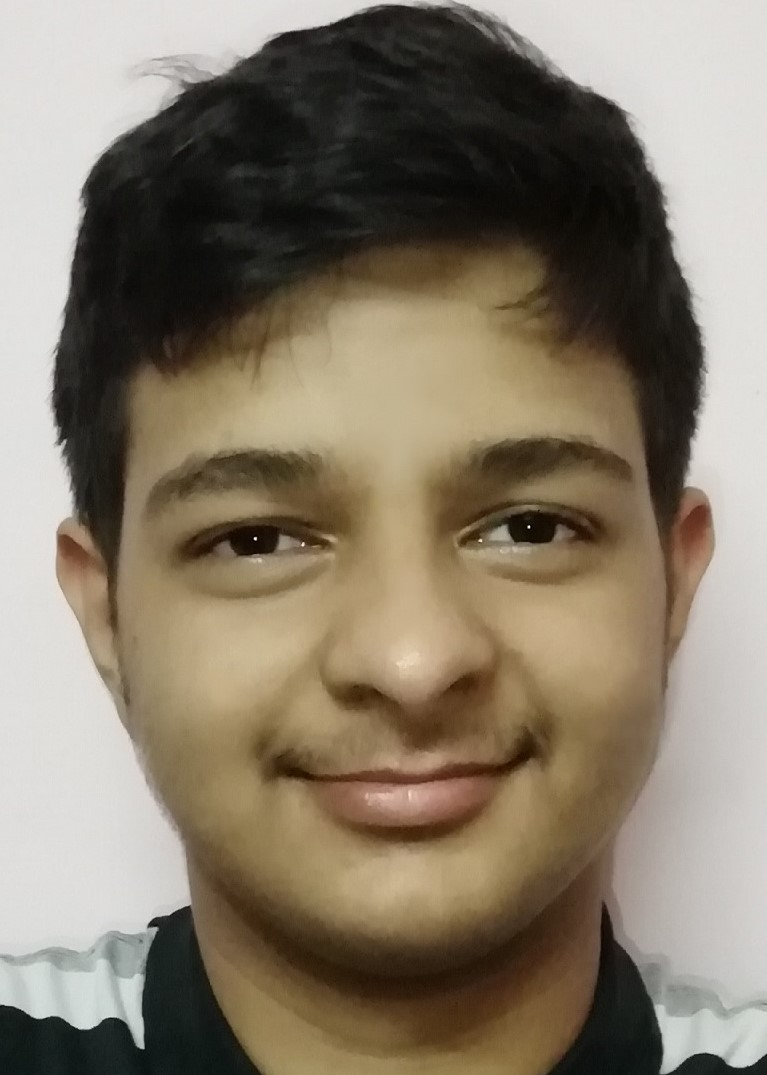
\includegraphics[scale = 0.08]{Swaraj.jpg}
\end{figure}
\section*{\textbf{CAREER OBJECTIVE}}
\noindent To have expert knowledge in Embedded Systems and be able to work in one of the top companies dealing with Embedded Systems.

\section*{\textbf{EDUCATION}}
\begin{tabular}{|c|c|c|c|c|}
\hline
Degree & College/School & University & Passing year & Pass percentage/CGPA\\
\hline
SSC & Gyan Kendra High School & Maharashtra State Board & 2015 & 93.2\%\\
\hline
HSC & Hansraj Morarji College of Science & Maharashtra State Board & 2017 & 86.15\%\\
\hline
B.Tech & Sardar Patel Institute& Autonomous affliated  & - &Sem\_1 - 8.96\\
 & of Technology & to Mumbai University & & Sem\_2 - 8.74\\
&&&&Sem\_3 - 9.58\\
\hline 
\end{tabular}


\section*{\textbf{PROJECTS}}
\begin{itemize}
\item Line following bot using Arduino.
\item Pulse rate sensor using Arduino.
\end{itemize}

\section*{\textbf{TRAINING AND INTERNSHIP}}
\begin{itemize}
\item Recieved training in embeded systems by SafeTTy systems.
\end{itemize}

\section*{\textbf{TECHNICAL SKILLS}}
\begin{itemize}
\item C.
\item Python (OpenCv, OpenGL).
\item Embedded C (Time triggered systems, Co-operative and hybrid schedulers).
\item IoT using MQTT protocol.
\item Autocad.
\item Blender.
\end{itemize}


\section*{\textbf{SOFT SKILLS}}
\begin{itemize}
\item Good communication.
\item Adaptability.
\item Teamwork.
\end{itemize}


\section*{\textbf{EXTRA-CURRICULAR ACTIVITIES}}
\begin{itemize}
\item Attended weekly Yoga clases conducted by Sardar Patel Institute of Technology. 
\item Active participation in Beach clean conducted by Afroz shah.
\item Organised an event named "Chain Reaction" for cultural fest "Ruminate '17" of Sardar Patel Institute of Technology.
\end{itemize}


\section*{\textbf{CO-CURRICULAR ACTIVITIES}}
\begin{itemize}
\item Attended workshop on Line following bot.
\item Attended workshop on Arduino.
\item Attended workshop on AVR microcontroller.
\end{itemize}

\section*{\textbf{COMPETITIONS AND CERTIFICATES}}
\begin{itemize}
\item Finalist in Eyantra robotics national competition hosted by IIT Bombay.\\https://github.com/SwarajKaondal/Eyrc2018-19.git
\end{itemize}


\section*{\textbf{Personal details}}
Father's name: Sarvjit Singh Kaondal\\
Mother's name: Saroj Kaondal\\
Nationality: Indian\\
Marital Status: Unmarried


\section*{\normalsize{\textbf{Reference:}}}
\noindent 
Prof. Dayanand Ambawade, Sardar Patel Institute of Technology \\e-mailid: dd\_ambawade@spit.ac.in


\section*{\textbf{\normalsize{Declaration:}}}
\noindent
 I hereby declare that the information furnished above is true to the best of my knowledge.


\section*{\textbf{\normalsize{Date:}}}
\noindent
 17-04-2019 
\end{document}
\end{document}